\section{Sécurité \& intégration continue}
La seconde partie de mon stage a été majoritairement consacrée à l'amélioration du processus de CI au sein d'Alter Frame. Il y a beaucoup à dire sur le sujet, tant en fait que je n'ai fait qu'effleurer la surface de ce qui est possible, d'une part parce qu'il s'agit d'un secteur de l'informatique encore jeune et d'autre part parce que je me suis naturellement concentré sur l'aspect ``sécurité'' qui est loin d'être le seul intérêt de l'intégration continue.

\subsection{Le contexte : GitLab-CI}
L'intégration continue dans les projets d'Alter Frame se fait à l'aide d'un service proposé par la plateforme d'hébergement de projets informatiques GitLab\footnote{\url{https://about.gitlab.com/}}. Le service en question, GitLab-CI\footnote{\url{https://about.gitlab.com/features/gitlab-ci-cd/}}, propose de mettre en place de l'intégration continue sur les projets hébergés sur GitLab.

Au moment de mon arrivée chez Alter Frame la partie CI des projets consistait majoritairement en la compilation des projets et une analyse de code à l'aide d'un plugin SonarQube\footnote{\url{https://www.sonarqube.org/}}, mise en place depuis environ 2 ans.

Le principe est que les actions décrites ci-dessus, compilation et analyse de code, sont effectuées à chaque push sur le serveur GitLab. Ce fonctionnement peut ensuite être affiné, pour ne se produire que lorsqu'un tag git est pushé ou sur certaines branches (branche master, tag de release, etc).

Il n'y avait néanmoins pas de composante cybersécurité dans le processus de CI d'Alter Frame et c'est donc ce sur quoi je suis intervenu en priorité. Néanmoins, mon travail ne s'est pas limité à cela et j'ai aussi pu intervenir sur d'autres aspects du CI et améliorer l'existant.

\subsection{Les outils}
\subsubsection{ZAP : Zed Attack Proxy}
\begin{figure}
  {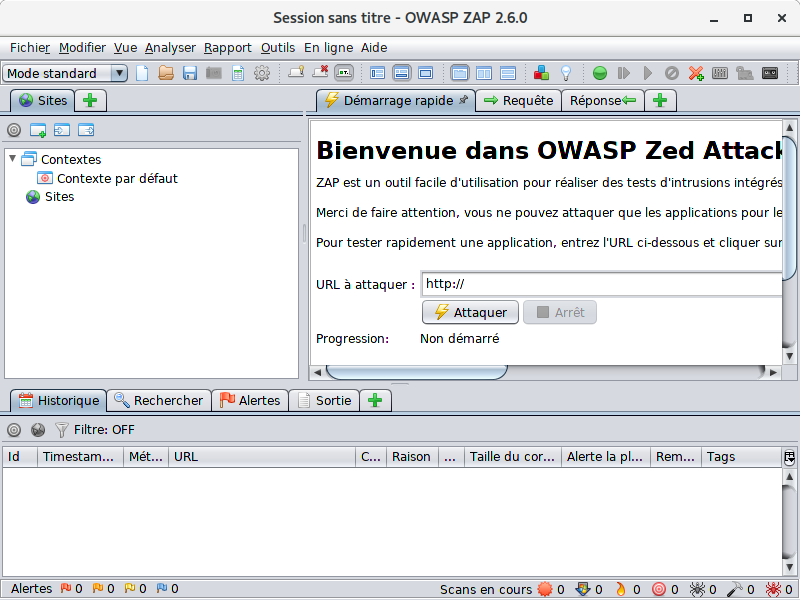
\includegraphics[width=\textwidth]{images/zap_acceuil}}
  \centering
  \caption{Fenêtre de démarrage de ZAP}
  \label{fig:zap_acceuil}
\end{figure}
ZAP\footnote{\url{https://www.owasp.org/index.php/OWASP_Zed_Attack_Proxy_Project}} (voir figure~\ref{fig:zap_acceuil}) est un projet open source développé par l'OWASP. Il s'agit un proxy qui peut intercepter et analyse le trafic qui traverse la machine hôte. ZAP est un outil de sécurité très intéressant et ce pour un grand nombre de raisons :
\begin{itemize}[label=$\bullet$]
\item activement développé\footnote{Plus de 60 commits en juin 2017, voir \url{https://github.com/zaproxy/zaproxy}} ;
\item open source et cross-platform ;
\item OWASP est une référence dans le monde de la sécurité ;
\item une large communauté, et donc une grande quantité de ressources sur laquelle s'appuyer ;
\item ZAP est contrôlable en ligne de commande/\textit{via} des APIs en plusieurs langages.
\end{itemize}

\begin{lstlisting}[language=bash, caption={Options de ZAP en ligne de commande},frame=single mv]
\$ zap.sh -cmd -help
	zap.sh [Options]

Options de base:
	-newsession <path>       Cree une nouvelle session a la position specifiee

	-session <path>          Ouvre la session specifiee apres le demarrage de ZAP

	-host <host>             Ecrase l'hote du proxy designe dans le fichier de configuration

	-port <port>             Ecrase le port du proxy designe dans le fichier de configuration


Options pour accessoires:
	-script <script>         Script a demarrer en ligne de commande ou a charger dans l'interface graphique
	-addoninstall <addon>    Installer l'accessoire specifie depuis la foire aux modules ZAP
	-addoninstallall         Installer tous les accessoires disponibles depuis la foire aux modules de ZAP
	-addonuninstall <addon>  Desinstalle l'accessoire specifie
	-addonupdate             Mettre a jour tous les accessoires modifies depuis la foire aux modules de ZAP
	-addonlist               Afficher tous les accessoires installes
	-quickurl [target url]: L'URL a attaquer, p.ex. http://www.example.com
	-quickout [output filename]: Le fichier dans lequel ecrire les resultats XML
	-quickprogress: Afficher les barres de progression pendant le balayage
\end{lstlisting}

Je n'avais, avant mon stage, que briévement eu l'occasion d'utiliser ZAP, au-travers du sous-projet de tests d'intrusion avec M. Pachy. Pouvoir m'entrainer plus longuement avec représentait donc à la fois un intérêt personnel, car cela me permettait d'en apprendre plus sur les vulnérabilités web les plus répandues, et professionnel car c'est un outil dont l'usage pourrait être pertinent pour mes futurs emplois.

\subsubsection{Docker}
Docker\footnote{\url{https://www.docker.com/}} est une technologie de virtualisation basée sur des conteneurs, qui vient se place en opposition aux hyperviseurs et machines virtuelles\footnote{Ou VMs pour Virtual Machines}. En plus d'une charte graphique à base de faune marine des plus plaisantes\footnote{\url{https://www.docker.com/sites/default/files/group_5622_0.png}}, la technologie Docker présente plusieurs fonctionnalités qui la rendent intéressante dans le monde de l'industrie informatique :
\begin{itemize}[label=$\bullet$]
\item un conteneur est plus léger qu'une VM ;
\item un conteneur s'exécute de la même façon sur n'importe quelmachine où Docker est installé ;
\item un conteneur peut embarquer toute la configuration nécessaire au bon fonctionnement de l'application, et c'est là le point le plus important. L'étape de configuration de l'environnement n'a à être effectuée qu'une seule fois, à la création de l'image\footnote{On ne parle de conteneur qu'une fois l'image en cours d'exécution, cf. différence entre processus et programmme}. De plus le système de Docker Store\footnote{\url{https://store.docker.com/}}, proche de celui d'un gestionnaire de paquets, permet au client d'avoir facilement la dernière version possible d'un logiciel, encore une fois en s'abstractisant des changements de configuration qui vont avec la mise-à-jour.
\end{itemize}

On assiste donc à une généralisation de l'utilisation de Docker depuis sa première version en 2013, avec de nombreux cas d'utilsation\footnote{\url{https://www.airpair.com/docker/posts/8-proven-real-world-ways-to-use-docker}}, mais aussi à une multiplication des outils en lien avec la technologie Docker comme des outils de gestion de groupes de containers\footnote{e.g. \href{https://kubernetes.io/}{Kubernetes}, \href{https://docs.docker.com/engine/swarm/}{Docker Swarm}}.

\subsubsection{YAML}
YAML Ain't Markup Language\footnote{\url{http://yaml.org/}}, de son nom complet, est un ``standard de serialisation de données''.

\subsection{Mon action sur le sujet}